\documentclass[border=10pt]{standalone}
\usepackage[svgnames]{xcolor}
\usepackage{amsmath}
\usepackage{pgfplots}
\pgfplotsset{compat=newest}
\usepackage[sfdefault]{FiraSans}
\usepackage{FiraMono}
\renewcommand*\familydefault{\sfdefault}
\begin{document}
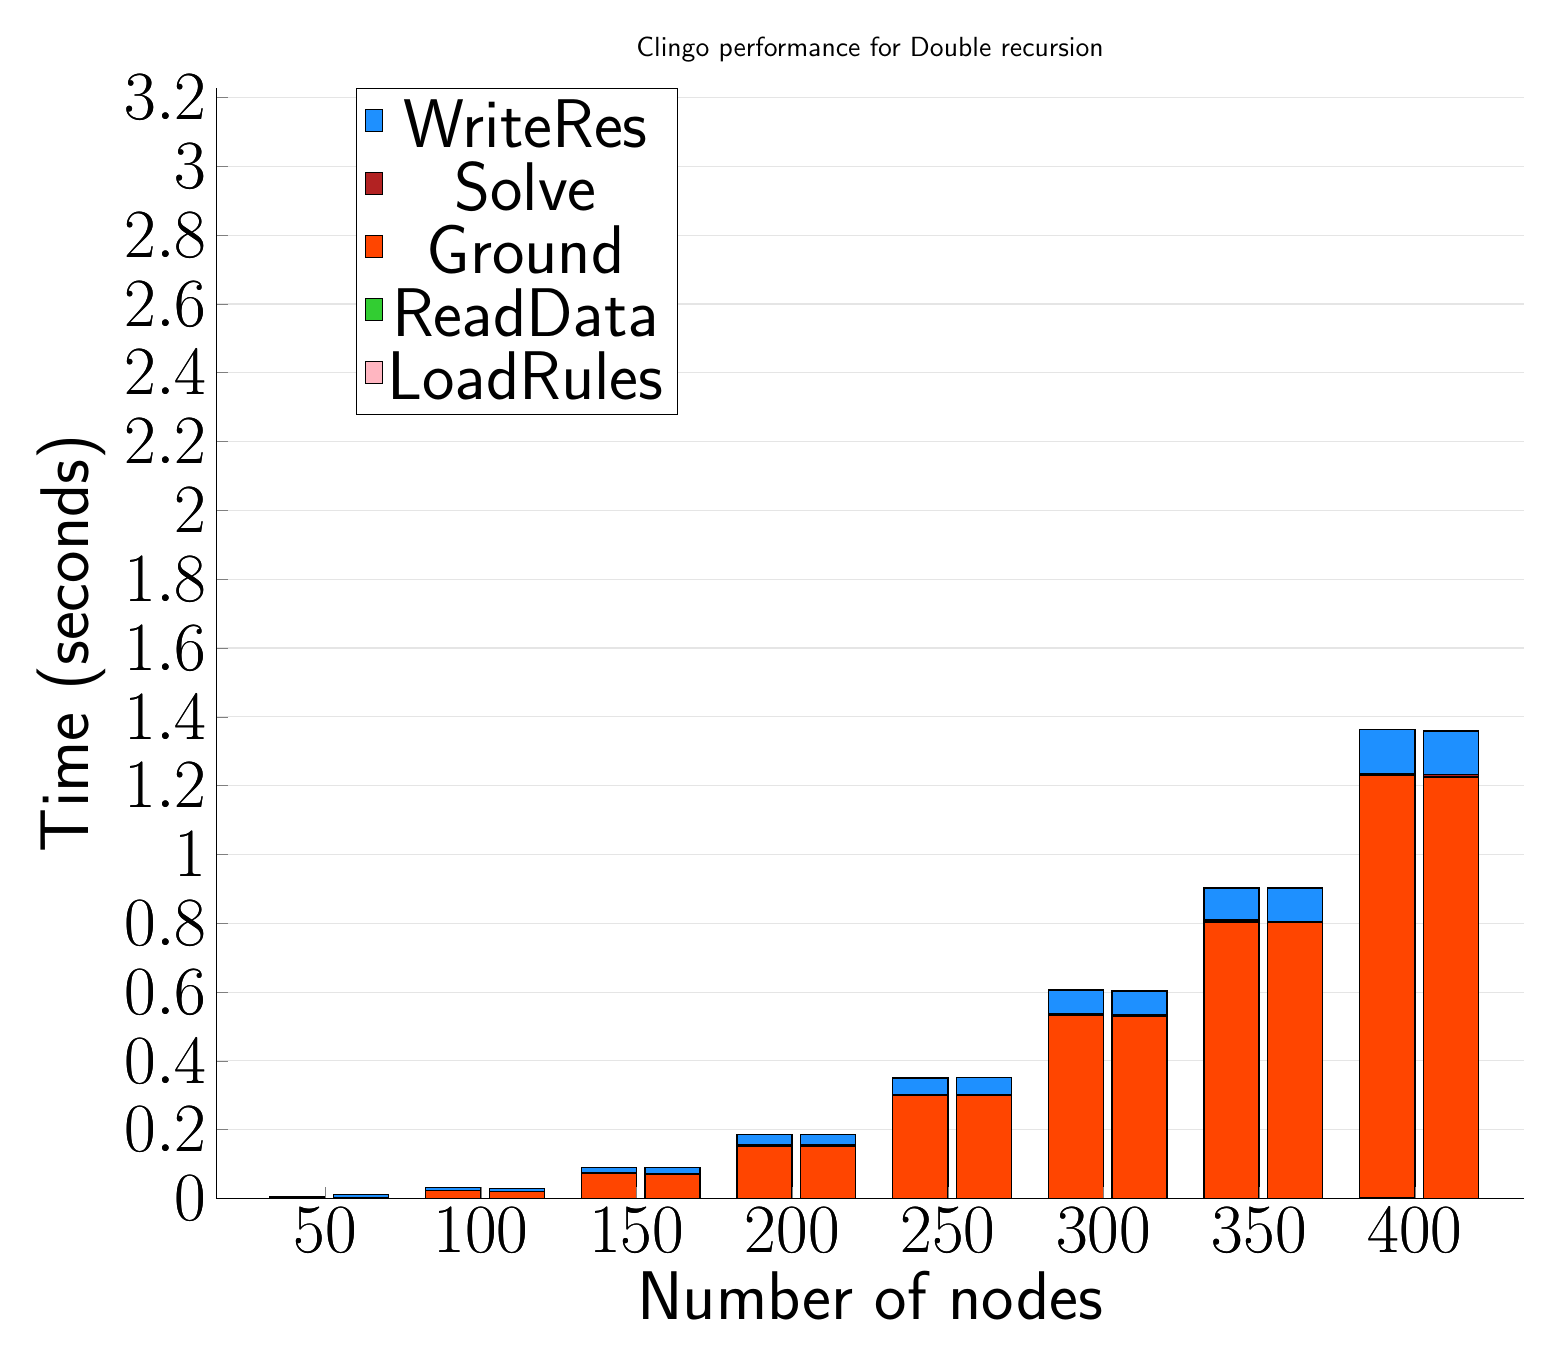
\begin{tikzpicture}
	\begin{axis}[
			ybar stacked,
			title={Clingo performance for Double recursion},
			bar shift=-10pt,
			width=1.5\textwidth,
			bar width=0.7cm,
			ymajorgrids, tick align=inside,
			major grid style={draw=gray!20},
			xtick=data,
			ymin=0, ymax=3.2279999971389772,
			axis x line*=bottom,
			axis y line*=left,
			enlarge x limits=0.1,
			legend style={
					at={(0.23, 1)},
					anchor=north,
					legend columns=1,
					font=\Huge,
				},
			ylabel={Time (seconds)},
			xlabel={Number of nodes},
			label style={font=\Huge},
			tick label style={font=\Huge},
		]
		\addlegendimage{fill=DodgerBlue, draw=black, line width=0.2pt}
		\addlegendentry{WriteRes}
		\addlegendimage{fill=FireBrick, draw=black, line width=0.2pt}
		\addlegendentry{Solve}
		\addlegendimage{fill=OrangeRed, draw=black, line width=0.2pt}
		\addlegendentry{Ground}
		\addlegendimage{fill=LimeGreen, draw=black, line width=0.2pt}
		\addlegendentry{ReadData}
		\addlegendimage{fill=LightPink, draw=black, line width=0.2pt}
		\addlegendentry{LoadRules}
		\addplot +[fill=LightPink, draw=black, line width=0.5pt] coordinates {
				(50, 0.0)
				(100, 0.0)
				(150, 0.0)
				(200, 0.0)
				(250, 0.0)
				(300, 0.0)
				(350, 0.0)
				(400, 0.0)
			};
		\addplot +[fill=LimeGreen, draw=black, line width=0.5pt] coordinates {
				(50, 0.0)
				(100, 0.0009999990463256836)
				(150, 0.0)
				(200, 0.0)
				(250, 0.0009999990463256836)
				(300, 0.0)
				(350, 0.0009999990463256836)
				(400, 0.0029999971389770507)
			};
		\addplot +[fill=OrangeRed, draw=black, line width=0.5pt] coordinates {
				(50, 0.003000020980834961)
				(100, 0.02200000286102295)
				(150, 0.0739999532699585)
				(200, 0.15299999713897705)
				(250, 0.2990000247955322)
				(300, 0.5319999933242798)
				(350, 0.8029999971389771)
				(400, 1.227999997138977)
			};
		\addplot +[fill=FireBrick, draw=black, line width=0.5pt] coordinates {
				(50, 0.0)
				(100, 0.0010000228881835937)
				(150, 0.0009999990463256836)
				(200, 0.0029999971389770507)
				(250, 0.0029999971389770507)
				(300, 0.0039999961853027345)
				(350, 0.005999994277954101)
				(400, 0.0039999961853027345)
			};
		\addplot +[fill=DodgerBlue, draw=black, line width=0.5pt] coordinates {
				(50, 0.0029999971389770507)
				(100, 0.009000015258789063)
				(150, 0.015999984741210938)
				(200, 0.02999999523162842)
				(250, 0.04699997901916504)
				(300, 0.0700000524520874)
				(350, 0.09300000667572021)
				(400, 0.12900002002716066)
			};
	\end{axis}
	\begin{axis}[
			ybar stacked,
			bar shift=13pt,
			width=1.5\textwidth,
			bar width=0.7cm,
			ymajorgrids, tick align=inside,
			major grid style={draw=none},
			xtick=data,
			ymin=0, ymax=3.2279999971389772,
			axis x line*=none,
			axis y line*=none,
			enlarge x limits=0.1,
			label style={font=\Huge},
			tick label style={font=\Huge},
		]
		\addplot +[fill=LightPink, draw=black, line width=0.5pt] coordinates {
				(50, 0.0)
				(100, 0.0)
				(150, 0.0)
				(200, 0.0)
				(250, 0.0009999999999999998)
				(300, 0.0)
				(350, 0.0)
				(400, 0.0)
			};
		\addplot +[fill=LimeGreen, draw=black, line width=0.5pt] coordinates {
				(50, 0.0)
				(100, 0.0)
				(150, 0.0)
				(200, 0.0)
				(250, 0.0)
				(300, 0.0)
				(350, 0.0009999999999999998)
				(400, 0.0)
			};
		\addplot +[fill=OrangeRed, draw=black, line width=0.5pt] coordinates {
				(50, 0.0009999999999999998)
				(100, 0.019999999999999997)
				(150, 0.07099999999999998)
				(200, 0.15299999999999997)
				(250, 0.299)
				(300, 0.531)
				(350, 0.8009999999999999)
				(400, 1.225)
			};
		\addplot +[fill=FireBrick, draw=black, line width=0.5pt] coordinates {
				(50, 0.0009999999999999998)
				(100, 0.0)
				(150, 0.0)
				(200, 0.003999999999999992)
				(250, 0.0010000000000000009)
				(300, 0.0030000000000000027)
				(350, 0.003999999999999992)
				(400, 0.008000000000000007)
			};
		\addplot +[fill=DodgerBlue, draw=black, line width=0.5pt] coordinates {
				(50, 0.008999999999999998)
				(100, 0.010000000000000004)
				(150, 0.019000000000000006)
				(200, 0.030000000000000006)
				(250, 0.04999999999999999)
				(300, 0.06899999999999996)
				(350, 0.09700000000000006)
				(400, 0.12599999999999995)
			};
	\end{axis}
\end{tikzpicture}

\end{document}
